\documentclass[12pt]{article}
\usepackage[margin=1.0in]{geometry}
%\usepackage{psfig}
%\usepackage{graphics}
\usepackage{amsmath, amssymb}
\usepackage[pdftex]{graphicx}
\usepackage{graphicx}
\usepackage{epstopdf}
\usepackage{textgreek}

\begin{document}
\bibliographystyle{plain}
\title{\Huge{\bf ECE 8540 Analysis of tracking systems}\\ 
\\ 
\huge Lab 4 - Kalman Filter}\\
\author{\LARGE Rahil Modi\\
C14109603}
\maketitle
\clearpage
\section{Introduction}
In this lab we are expected to develop a code to design a Kalman filter. A set of sensor data is used to design a model. The model is used to smooth the noise and predict the future states to get them as close as to the actual measurement. The sensor data is random and not predictable that is the reason we will be tracking the sensor data to get a good estimate of the future states.\\In this lab we will be using 1D and 2D sensor data. This report includes the derivation of Kalman filter equations, plots of the results and discussion of the results. The dynamic noise to measurement noise ratio will be changed to study the behavior of the filter. Three different ratios are showed in the results.\\ The entire MATLAB code is in the appendix.
\section{Methods}
Kalman filter works on continuous cycle where the variables get updated with every loop. The various equations of implementation of Kalman filter are enlisted below.\\
1. Predict new state:
\begin{equation}
X_{t,t-1} = \Phi X_{t-1,t-1}
\end{equation}
2. Predict next state covariance:
\begin{equation}
S_{t,t-1} = \Phi S_{t-1,t-1}\Phi^T + Q
\end{equation}
3. Obtain measurement(s): $Y_t$\\
4. Calculate the Kalman gain:
\begin{equation}
K_t = S_{t, t-1}M^T[MS_{t,t-1}M^T+R]^{-1}
\end{equation}
5. Update state
\begin{equation}
X_{t,t} = X_{t,t-1}+K_t(Y_t-MX_{t,t-1})
\end{equation}
6. Update state covariance
\begin{equation}
S_{t,t} = [I - K_tM]S_{t,t-1}
\end{equation}
7. Loop (now $t$ becomes $t+1$)\\
\\
Where,\\
$X_t$ : current actual state\\
$X_{t+1}$ : next actual state\\
$\Phi$ : state transition matrix\\
\textit{S\textsubscript{t}} : state estimate covariance\\
\textit{Y\textsubscript{t}} : sensor measurement\\
\textit{K\textsubscript{t}} : kalman gain\\
\textit{Q} : dynamic noise matrix\\
\textit{R} : measurement noise matrix\\
\textit{M} : observation matrix\\
The two variables that need to be controlled are Q and R.\\

\subsection{Derivation of 1D model equations}
The above equations are implemented on a 1D constant velocity model to predict the position after time t = t+1.\\
1. State Variables:
\begin{equation}
X_t=
\[\begin{bmatrix}
x_t\\
\dot{x}_t
\end{bmatrix}\]
\end{equation}
where \textit{x\textsubscript{t}} is the position and \textit{\.{x}\textsubscript{t}} is velocity.\\
2. State Transition Equation:
\begin{equation}
x_{t,t} = X_{t,t-1} + \dot{X}_{t,t-1}T
\end{equation}
\begin{equation}
\dot{x}_{t,t} = \dot{X}_{t,t-1}
\end{equation}
where T is the time interval/sample time. T = 1 is assumed in our case. The state variable covariance is
$s_t$ = 
\begin{bmatrix}
	\sigma^2_{x_t} & \sigma_{x_t,\dot{x_t}} \\
	\sigma_{x_t,\dot{x_t}} & \sigma^2_{\dot{x_t}}
\end{bmatrix}}\\
3. State transition matrix:
\begin{equation}
X_{t+1} = \Phi X_t+A_t
\end{equation}
It can be written in the matrix form as:
\begin{equation}
\[\begin{bmatrix}
x_{t+1}\\
\dot{x}_{t+1}
\end{bmatrix} = \begin{bmatrix}
1&T\\
0&1
\end{bmatrix} \begin{bmatrix}
x_t\\
\dot{x}_t
\end{bmatrix} + \begin{bmatrix}
0\\
N(0, \sigma^2_a)
\end{bmatrix}\]
\end{equation}\\
where, \textit{N}(0, \textsigma\textsuperscript{2}\textsubscript{a}) = noise in acceleration over T and \textit{Q} = \textit{cov}[\textit{A}] = \begin{bmatrix}
0&0\\
0&\sigma^2_a
\end{bmatrix}\\
4. Measurement Equation:
\begin{equation}
Y_t = M * X_t + N_t
\end{equation}
\begin{equation}
\[\begin{bmatrix}
Y_t
\end{bmatrix} = \begin{bmatrix}
1&0
\end{bmatrix} \begin{bmatrix}
x_t\\
\dot{x}_t
\end{bmatrix} + \begin{bmatrix}
N(0,\sigma^2_n)
\end{bmatrix}\]
\end{equation}\\
where, \textit{N\textsubscript{t}} is the measurement noise and measurement noise covariance = \textit{R} = \textit{cov}[\textit{N}] \begin{bmatrix}
\sigma^2_n
\end{bmatrix}. M is the observation matrix and it is a constant velocity.\\
5. State predict equations:
\begin{equation}
X_{t+1} = \Phi X_{t}
\end{equation}
\begin{equation}
\[X_{t,t-1}=
\begin{bmatrix}
1&T\\
0&1
\end{bmatrix} X_{t-1,t-1}
\end{equation}\\
The \textit{X\textsubscript{t-1,t-1}} = [-0.3317 0] is taken which is the first sensor measurement data. It will get updated in the loop.\\
6. State update equations
\begin{equation}
X_{t,t} = X_{t,t-1} + K_t(Y_t - [1, 0] X_{t,t-1})
\end{equation}
where, \textit{K\textsubscript{t}} is the kalman gain.\\
The MATLAB Code for this part is given in the appendix section.\\
The results of this part are discussed in the section 3.1.

\subsection{Derivation of 2D model equations}
The derivation for a 2D constant velocity model is done below.\\
1. State Variables:\\
The state \textit{X\textsubscript{t}} is defined as:
\begin{equation}
X_t = 
\begin{bmatrix}
x_t \\
y_t \\
\dot{x}_t\\
\dot{y}_t
\end{bmatrix}
\end{equation}
where $x_t$ and $y_t$ is the position and $\dot{x}_t$ and $\dot{y}_t$ is the velocity.\\
2. State transition equations:
\begin{align}
\begin{split}
	X_{t+1} &= x_t + T \dot{x_t} \\
	\\
	Y_{t+1} &= y_t + T \dot{y_t} \\
	\\
	\dot{X_t} &=  \dot{x_t} \\
	\\
	\dot{Y_t} &=  \dot{y_t}
\end{split}
\end{align}\\
The state variable covariance is $s_t$ = 
\begin{bmatrix}
	\sigma^2_{x_t} & \sigma_{x_t,y_t} & \sigma_{x_t,\dot{x_t}} & \sigma_{x_t,\dot{y_t}}  \\
	\sigma_{x_t,y_t} & \sigma^2_{y_t} & \sigma_{y_t,\dot{x_t}} & \sigma_{y_t,\dot{y_t}} \\
	\sigma_{x_t,\dot{x_t}} & \sigma_{y_t,\dot{x_t}} & \sigma^2_{\dot{x_t}} & \sigma_{\dot{x_t},\dot{y_t}} \\
	\sigma_{x_t,\dot{y_t}} & \sigma_{y_t,\dot{y_t}} & \sigma_{\dot{x_t},\dot{y_t}} & \sigma^2_{\dot{y_t}}
\end{bmatrix}\\
3. State transition matrix
\begin{equation}
X_{t+1} = \Phi X_t+A_t
\end{equation}
It can be written as:
\begin{equation}
\[\begin{bmatrix}
x_{t+1} \\
y_{t+1} \\
\dot{x}_{t+1}\\
\dot{y}_{t+1}
\end{bmatrix} = \begin{bmatrix}
	1 & 0 & T & 0 \\
	0 & 1 & 0 & T \\
	0 & 0 & 1 & 0 \\
	0 & 0 & 0 & 1
\end{bmatrix} \begin{bmatrix}
x_t \\
y_t \\
\dot{x}_t\\
\dot{y}_t
\end{bmatrix} + \begin{bmatrix}
	0 \\
	0 \\
	N(0,\sigma^2_{a1}) \\
	N(0,\sigma^2_{a2})
\end{bmatrix}\]
\end{equation}\\
Covariance in dynamic noise will be $Q$ = $cov$[$A$] = \begin{bmatrix}
	0 & 0 & 0 & 0\\
	0 & 0 & 0 & 0\\
	0 & 0 & \sigma^2_{a_1} & \sigma_{a_1,a_2} \\
	0 & 0 & \sigma_{a_1,a_2} & \sigma^2_{a_2}
\end{bmatrix}\\
4. Measurement equation:
\begin{equation}
Y_t = M * X_t + N_t
\end{equation}
It can be written as:
\begin{equation}
\[Y_t = 
\begin{bmatrix}
	\tilde{x_t} \\
	\tilde{y_t}
\end{bmatrix} =
\begin{bmatrix}
	1 & 0 & 0 & 0 \\
	0 & 1 & 0 & 0
\end{bmatrix} \begin{bmatrix}
x_t \\
y_t \\
\dot{x}_t\\
\dot{y}_t
\end{bmatrix} + \begin{bmatrix}
	N(0,\sigma^2_{n1}) \\
	N(0,\sigma^2_{n2})
\end{bmatrix}
\end{equation}\\
Measurement noise covariance = $R$ = $cov$[$N$] = \begin{bmatrix}
	\sigma^2_{n_1} & \sigma_{n_1,n_2} \\
	\sigma_{n_1,n_2} & \sigma^2_{n_2} 
\end{bmatrix}\\
5. State predict equations:
\begin{equation}
X_{t+1} = \Phi X_{t}
\end{equation}
\begin{equation}
\[X_{t,t-1}=
\begin{bmatrix}
	1 & 0 & T & 0 \\
	0 & 1 & 0 & T \\
	0 & 0 & 1 & 0 \\
	0 & 0 & 0 & 1
\end{bmatrix} X_{t-1,t-1}
\end{equation}\\
The \textit{X\textsubscript{t-1,t-1}} = [274.15 660.70] is taken which is the first sensor measurement data. It will get updated in the loop.\\
6. State update equations:
\begin{equation}
X_{t,t} = X_{t,t-1} + K_t(Y_t - \begin{bmatrix}
	1 & 0 & 0 & 0 \\
	0 & 1 & 0 & 0
\end{bmatrix} X_{t,t-1})
\end{equation}
where, \textit{K\textsubscript{t}} is the kalman gain.\\
The MATLAB Code for this part is given in the appendix section.\\
The results of this part are discussed in the section 3.2.

\section{Results}
\subsection{For first data set}
The plots below show the results of the 3 dynamic noise to measurement noise ratios. For the 1D constant velocity model the dynamic noise Q is kept fixed at 0.01 and the measurement noise R is varied.\\
Ratio 1:\\
Measurement Noise (R) = 1\\
Dynamic Noise (Q) = 0.001\\
\centerline{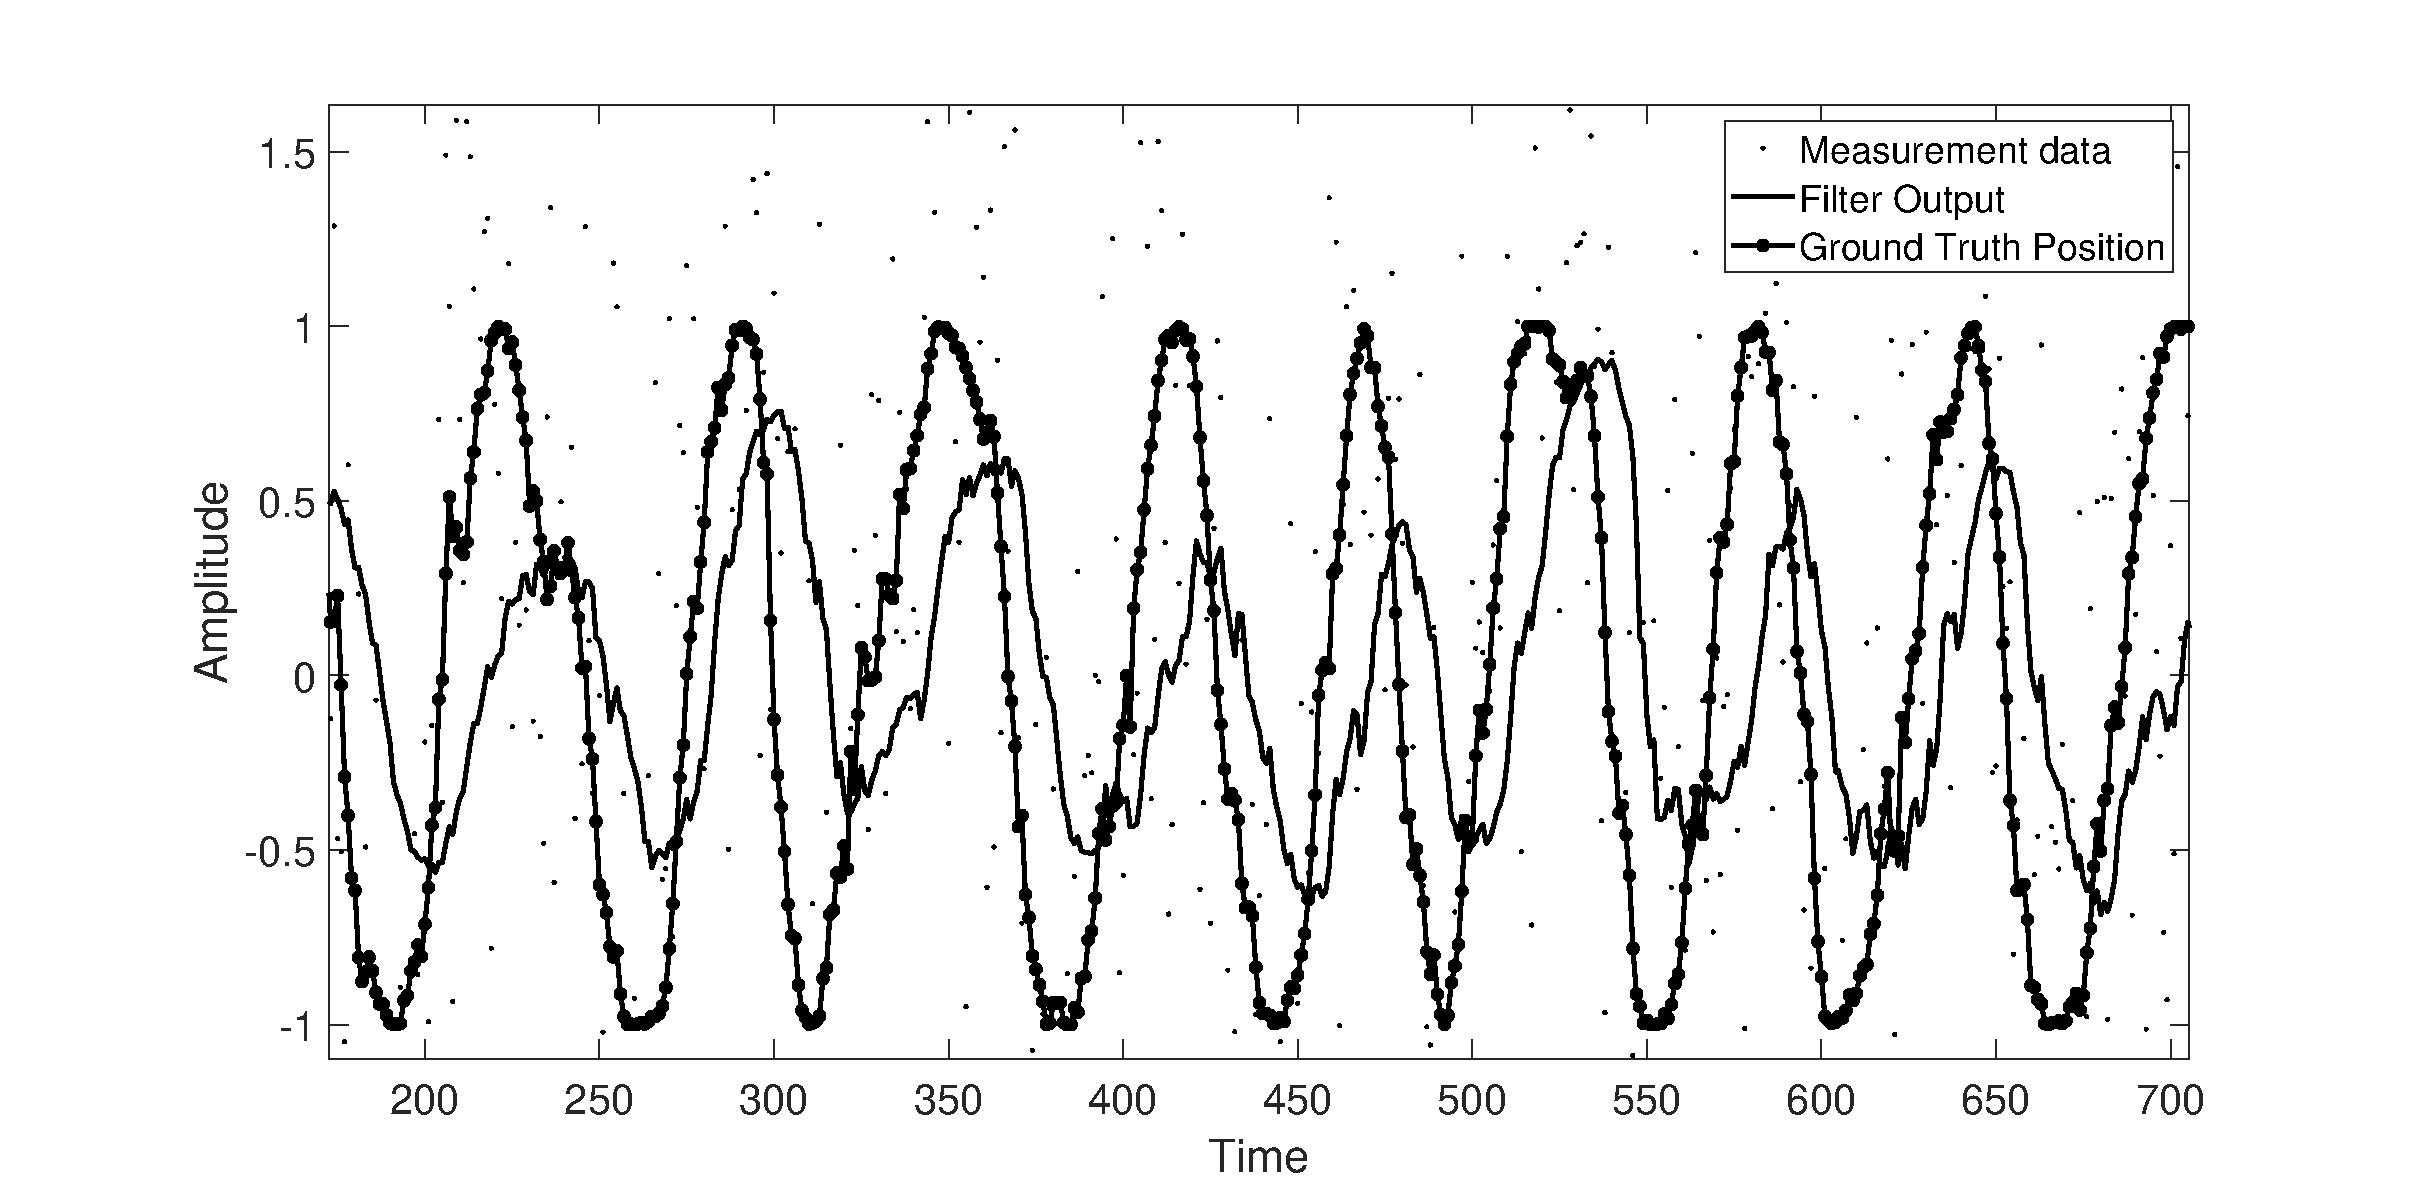
\includegraphics[scale=0.5]{1.eps}}
\centerline{\caption{Figure 1: Kalman filter 1D plot for Ratio 1}}\\
\centerline{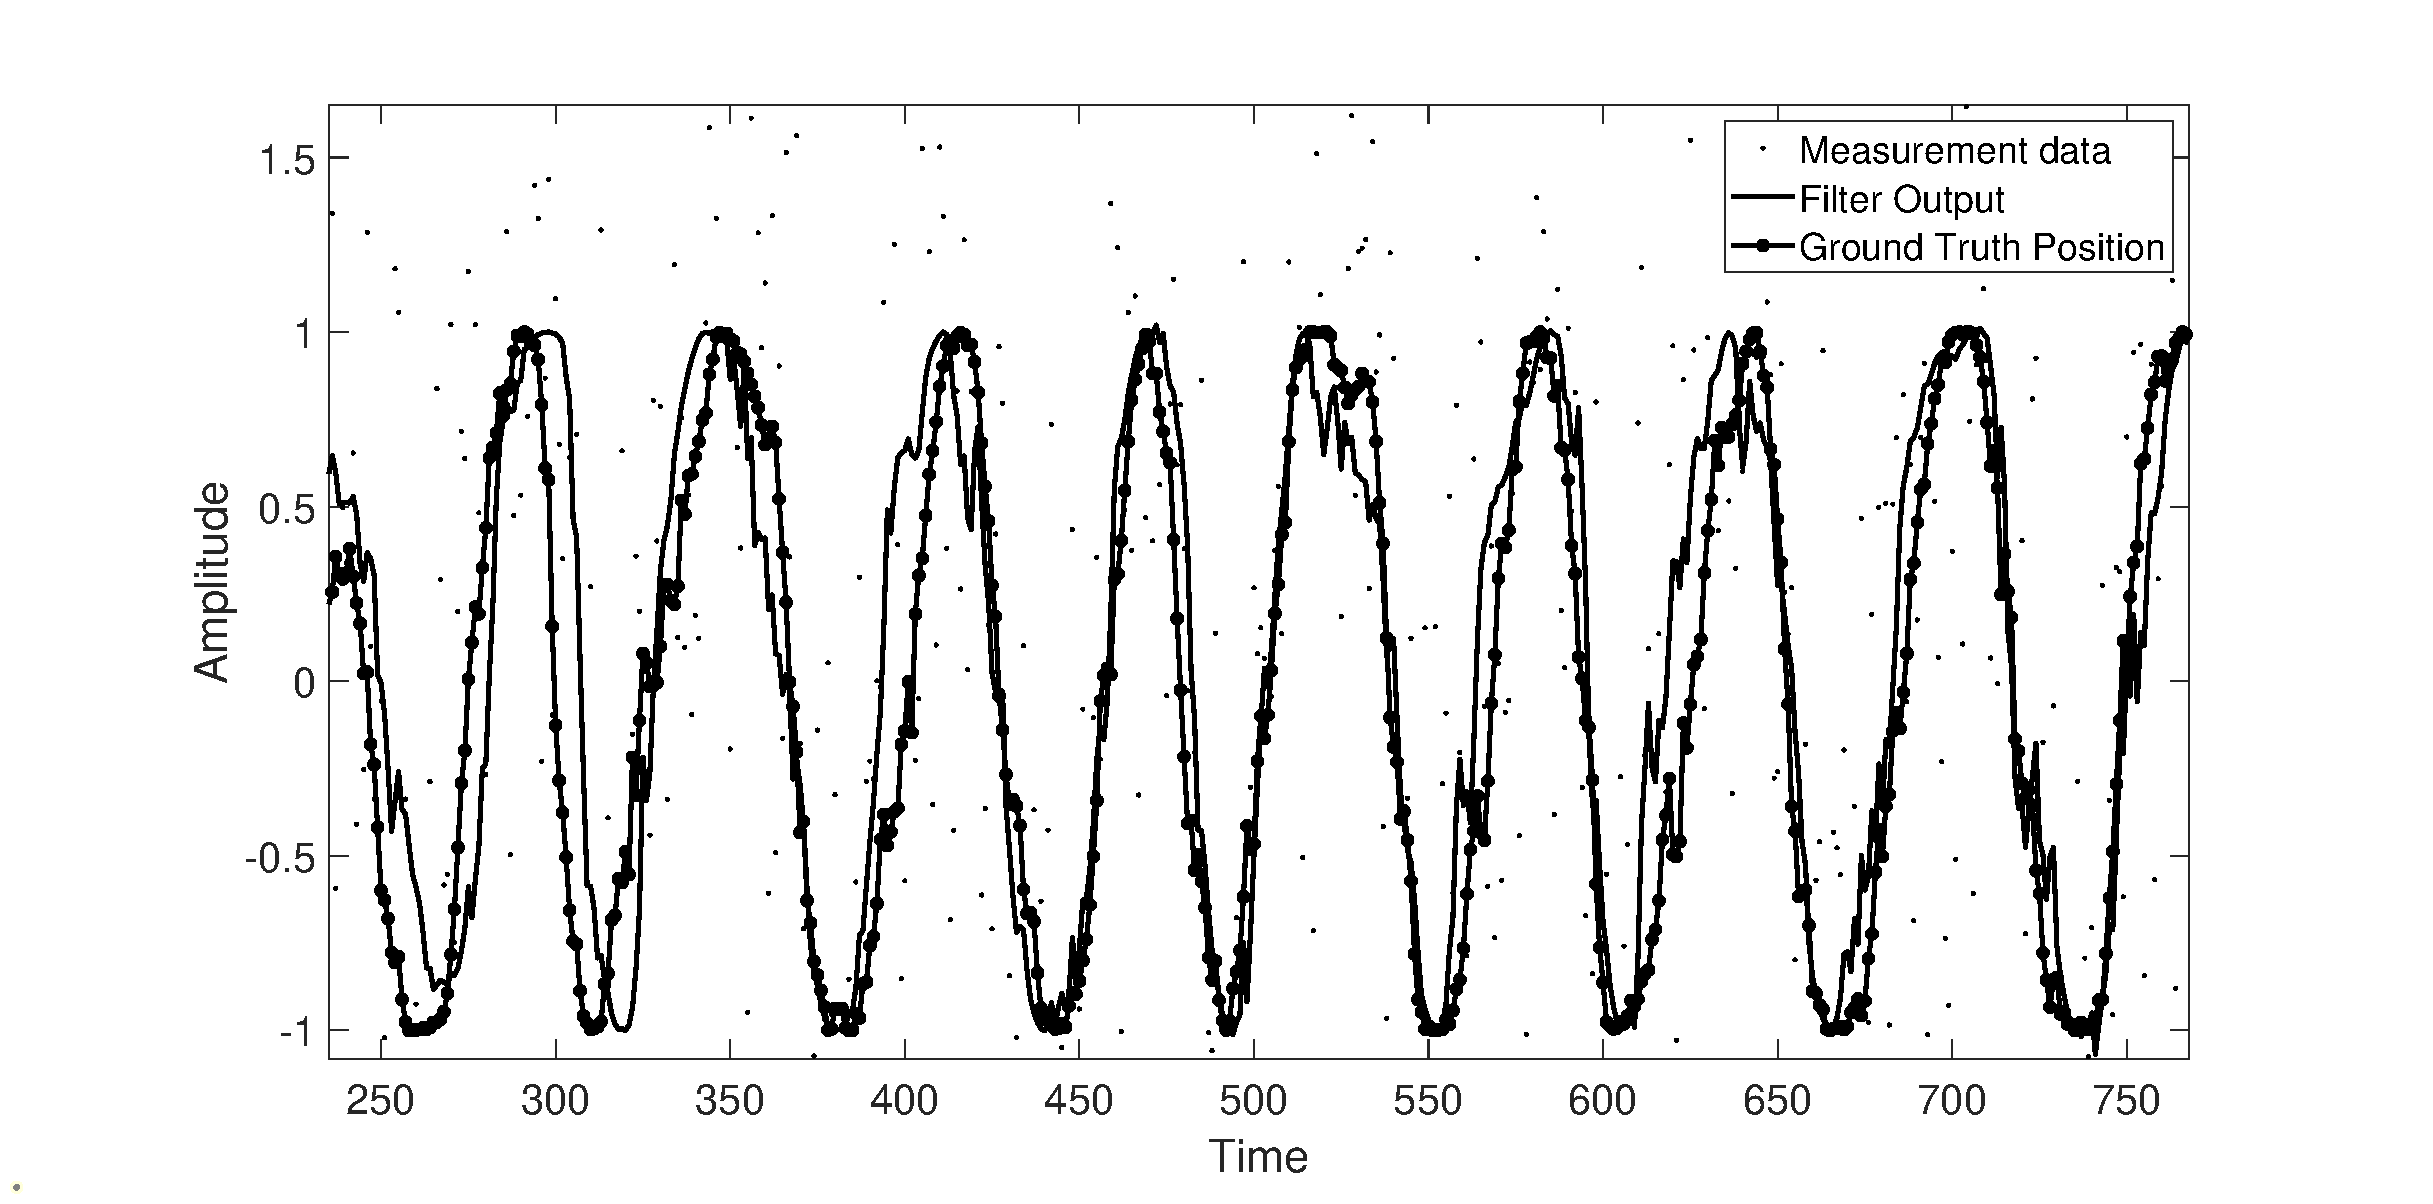
\includegraphics[scale=0.5]{2.eps}}
\centerline{\caption{Figure 2: Zoomed Kalman filter 1D plot for Ratio 1}}\\
Ratio 2:\\
Measurement Noise (R) = 1\\
Dynamic Noise (Q) = 10\\
\centerline{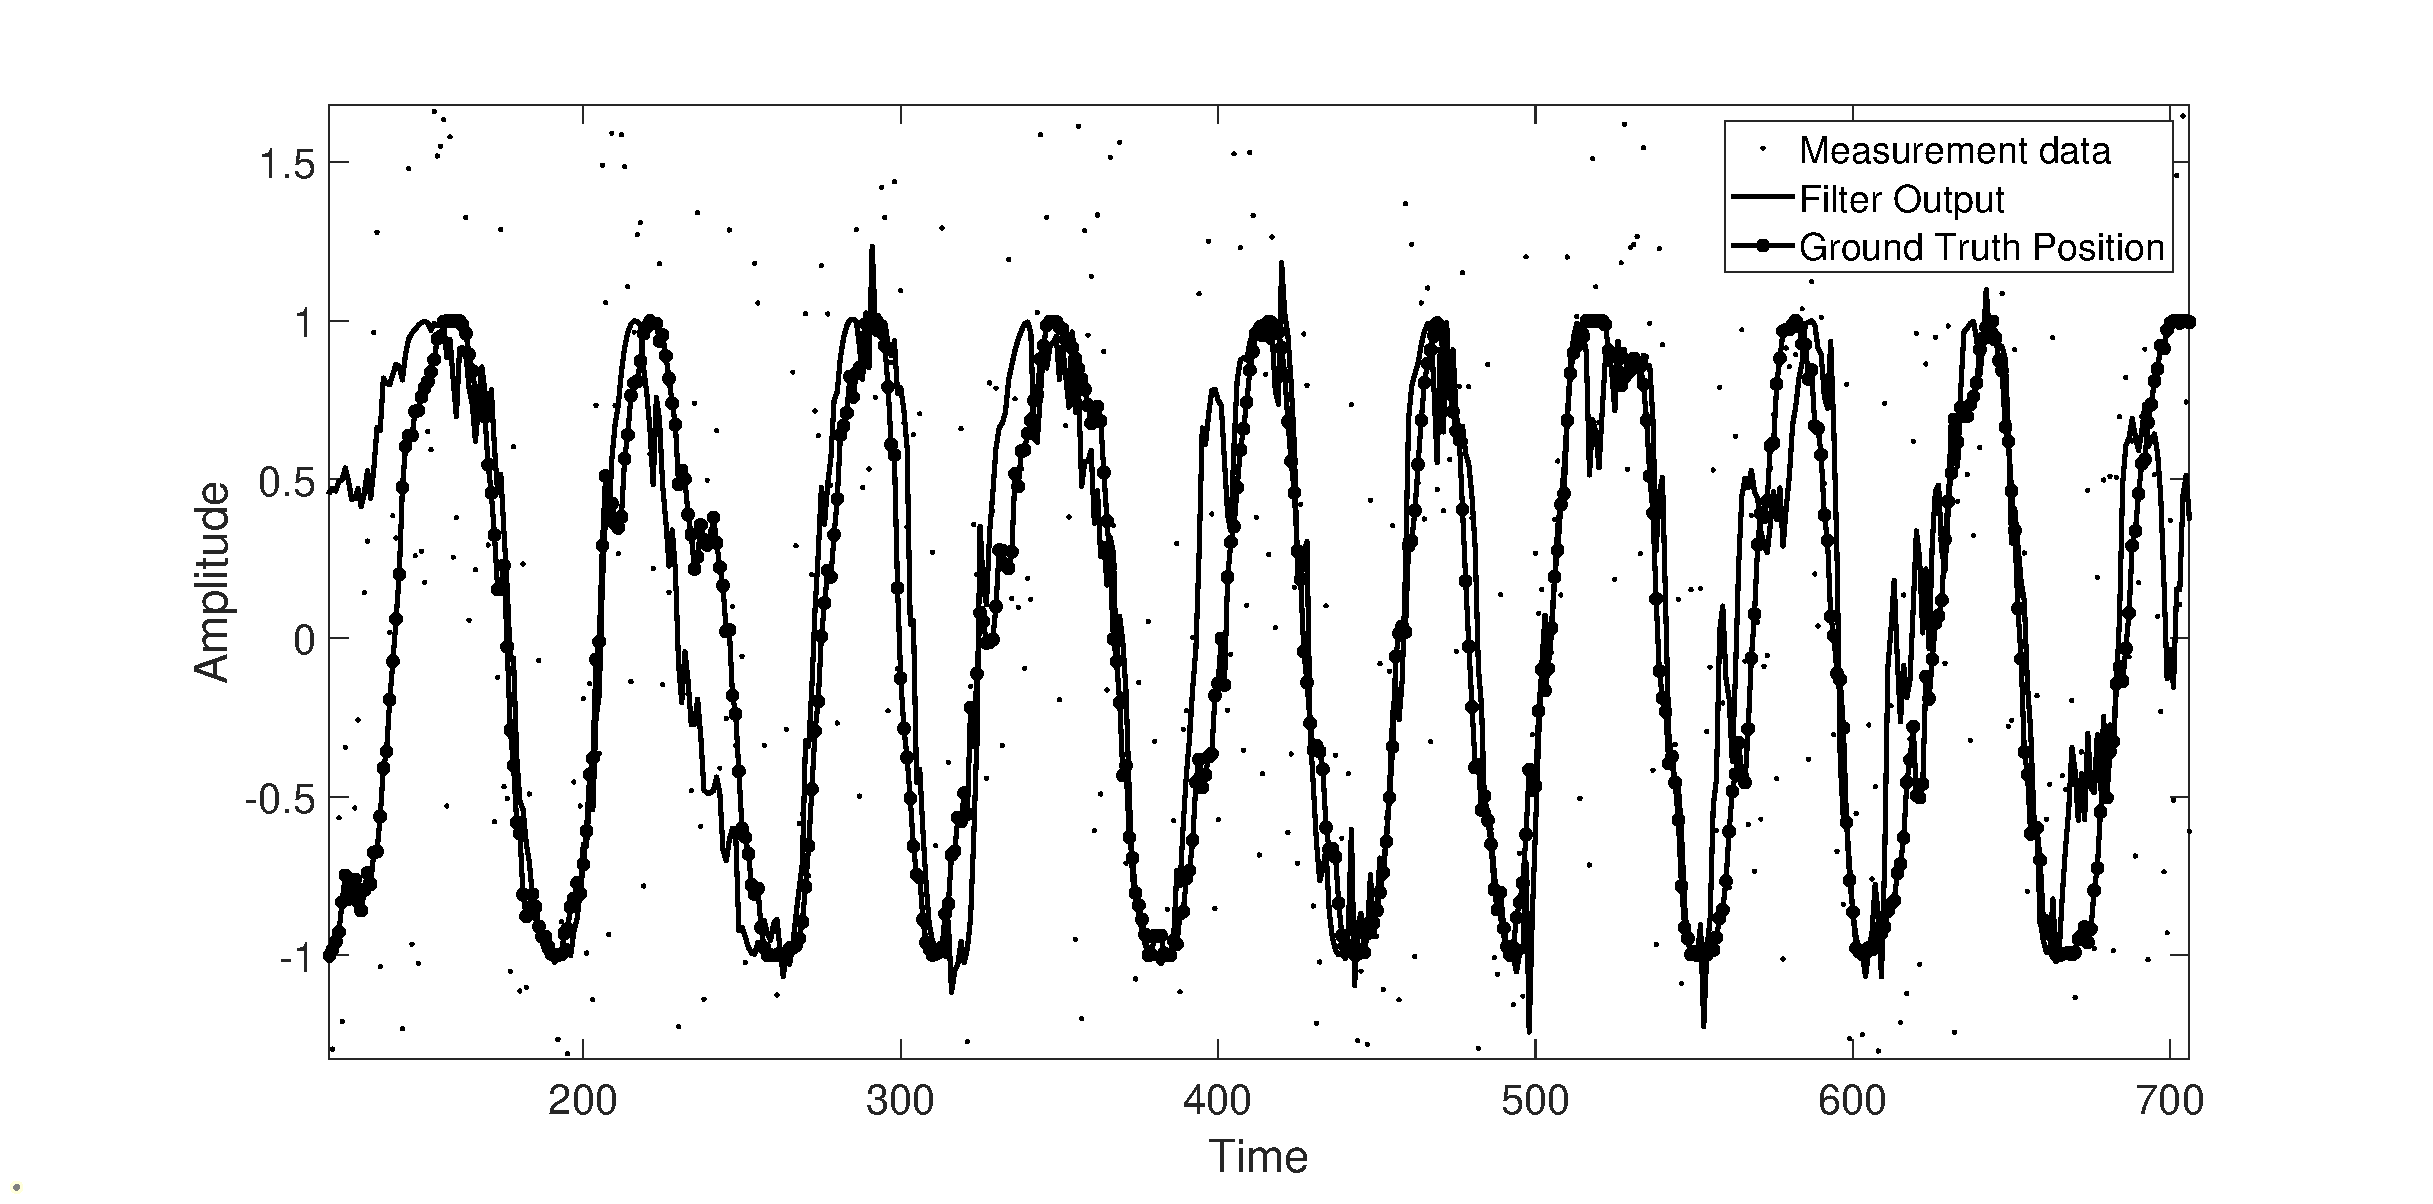
\includegraphics[scale=0.5]{3.eps}}
\centerline{\caption{Figure 3: Kalman filter 1D plot for Ratio 2}}\\
\centerline{\includegraphics[scale=0.5]{4.eps}}
\centerline{\caption{Figure 4: Zoomed Kalman filter 1D plot for Ratio 2}}\
Ratio 3\\
Measurement Noise (R) = 1\\
Dynamic Noise (Q) = 0.000001\\
\centerline{\includegraphics[scale=0.5]{5.eps}}
\centerline{\caption{Figure 5: Kalman filter 1D plot for Ratio 3}}\\
\centerline{\includegraphics[scale=0.5]{6.eps}}
\centerline{\caption{Figure 6: Zoomed Kalman filter 1D plot for Ratio 3}}\
Reducing the Dynamic noise the predicted values will shift away from the measurement values as we would be trusting our predicted values more than the measurement values. It can be observed in figure 2 when the Q is large the values are very close to the measurement values. It can be observed in figure 3 when the Q values decreases the predicted value keeps on moving away from the measurement value. The figure 1 shows a balance between Q and R values which compensates for the not being centered at measurements or averaged in measurements and not containing a lot of noise.
\subsection{For second data set}
The plots below show the results of the 3 dynamic noise to measurement noise ratios. For the 2D constant velocity model the measurement noise R is kept fixed at 1 and the dynamic noise Q is varied.\\
Ratio 1:\\
Measurement Noise (R) = 0.1\\
Dynamic Noise (Q) = 0.01\\
\centerline{\includegraphics[scale=0.5]{7.eps}}
\centerline{\caption{Figure 7: Kalman filter 2D X position plot for Ratio 1}}\\
\centerline{\includegraphics[scale=0.5]{8.eps}}
\centerline{\caption{Figure 8: Zoomed Kalman filter 2D X position plot for Ratio 1}}\\
\centerline{\includegraphics[scale=0.5]{9.eps}}
\centerline{\caption{Figure 9: Kalman filter 2D Y position plot for Ratio 1}}\\
\centerline{\includegraphics[scale=0.5]{10.eps}}
\centerline{\caption{Figure 10: Zoomed Kalman filter 2D Y position plot for Ratio 1}}\\
Ratio 2:\\
Measurement Noise (R) = 100\\
Dynamic Noise (Q) = 0.01\\
\centerline{\includegraphics[scale=0.5]{11.eps}}
\centerline{\caption{Figure 11: Kalman filter 2D X position plot for Ratio 2}}\\
\centerline{\includegraphics[scale=0.5]{12.eps}}
\centerline{\caption{Figure 12: Zoomed Kalman filter 2D X position plot for Ratio 2}}\\
\centerline{\includegraphics[scale=0.5]{13.eps}}
\centerline{\caption{Figure 13: Kalman filter 2D Y position plot for Ratio 2}}\\
\centerline{\includegraphics[scale=0.5]{14.eps}}
\centerline{\caption{Figure 14: Zoomed Kalman filter 2D Y position plot for Ratio 2}}\\
Ratio 3\\
Measurement Noise (R) = 0.000001\\
Dynamic Noise (Q) = 0.01\\
\centerline{\includegraphics[scale=0.5]{15.eps}}
\centerline{\caption{Figure 15: Kalman filter 2D X position plot for Ratio 3}}\\
\centerline{\includegraphics[scale=0.5]{16.eps}}
\centerline{\caption{Figure 16: Zoomed Kalman filter 2D X position plot for Ratio 3}}\\
\centerline{\includegraphics[scale=0.5]{17.eps}}
\centerline{\caption{Figure 17: Kalman filter 2D X position plot for Ratio 3}}\\
\centerline{\includegraphics[scale=0.5]{18.eps}}
\centerline{\caption{Figure 18: Zoomed Kalman filter 2D X position plot for Ratio 3}}\\
Reducing the measurement noise pushes the predicted values towards the measurement values. It can be observed that decreasing the R moves the predicted values towards to the measurement values. For this part I have fixed the Q value at 0.01 and measurement noise R is varied. 
\section{Conclusion}
We have learned from this lab about Kalman filtering, how to derive the equations for the 1D and 2D problems. I have also learned that Q and R are the control knobs of the Kalman Filter. Tuning them will result in a better performing kalman filter. Reducing Q value shifts the predicted values away from the measurement values which says you trust your predicted values more. Reducing R value shifts the predicted values towards the measurement values which says you trust the measurement values more than your predicted values. A proper ratio is needed to be determined for better performing kalman filter. 
\section{Appendix}
\begin{verbatim}
%% Part 1
clc
clear all
close all
A = importdata('1D-data.txt');

T = 1;                 %Sample Time/ Time Interval
R = 1;                 %Measurement noise
q = 0.000001;              %Dynamic Noise

psi       = [1 T;
             0 1];                % State Transition Matrix
M         = [1 0];                % Observation Matrix
X_prev    = [-0.3317; 
                  0];             % Previous State matrix
Q         = [0 0; 
             0 q];                % Dynamic noise covariance
S_prev    = [1 0; 
             0 1];                % State covariance
pred_data = zeros(1, length(A));  % Output


for i = 1 : length(A)
    Yt(i)        = A(i);                 % Sensor Measurement
    X_next       = psi * X_prev;
    S_next       = (psi * S_prev * psi') + Q;
    Kt           = S_next * M'/((M * S_next * M') + R);
    X_update     = X_next + (Kt * (Yt(i) - M * X_next));
    S_update     = (eye(2) - Kt * M) * S_next;
    pred_data(i) = X_update(1,1);
    X_prev       = X_update;
    S_prev       = S_update;
end 

figure
X = 1:length(A);
hold on
%axis([100 190 -3 3])
plot(X, A, 'k');
plot(X, pred_data, 'k.-', 'markersize',10, 'linewidth', 1.5);
xlabel("Sampling Time (T)");
ylabel("Position (Xt)");
legend("Measured Values", "Predicted Values");
hold off

%% Part 2
clc
clear all
close all

A = importdata('2D-UWB-data.txt');

T = 1;                 %Sample Time/ Time Interval
r = 0.000001;             %Measurement noise
q = 0.01;             %Dynamic Noise

psi       = [1 0 T 0;
             0 1 0 T;
             0 0 1 0;
             0 0 0 1];            % State Transition Matrix
M         = [1 0 0 0;
             0 1 0 0];            % Observation Matrix
X_prev    = [A(1,1); 
             A(1,2);
                  0;
                  0];             % Previous State matrix
R         = [r 1;
             1 r];                % Measurement noise covariance
Q         = [0 0 0 0; 
             0 0 0 0; 
             0 0 q 1; 
             0 0 1 q];            % Dynamic noise covariance
S_prev    = [1 0 0 0; 
             0 1 0 0;
             0 0 1 0;
             0 0 0 1];                % State covariance
pred_data = zeros(2, length(A(:,1)));  % Output
Yt = A';

for i = 1 : length(A)
    X_next       = psi * X_prev;
    S_next       = (psi * S_prev * psi') + Q;
    Kt           = S_next * M'/((M * S_next * M') + R);
    X_update     = X_next + (Kt * (Yt(:,i) - M * X_next));
    S_update     = (eye(4) - Kt * M) * S_next;
    pred_data(1,i) = X_update(1,1);
    pred_data(2,i) = X_update(2,1);
    X_prev       = X_update;
    S_prev       = S_update;
end 

figure
X = 1:length(A);
hold on
plot(X, A(:,1), 'k');
plot(X, pred_data(1,:), 'k.-','markersize',10, 'linewidth', 1.5);
xlabel("Sampling Time (T)");
ylabel("Position (Xt)");
legend("Measured Values", "Predicted Values");
hold off

figure
X = 1:length(A);
hold on
plot(X, A(:,2), 'k');
plot(X, pred_data(2,:), 'k.-', 'markersize',10, 'linewidth', 1.5);
xlabel("Sampling Time (T)");
ylabel("Position (Xt)");
legend("Measured Values", "Predicted Values");
hold off
\end{verbatim}
\end{document}